\documentclass[a4paper]{article}
\usepackage[T1]{fontenc}			% \chapter package
\usepackage[english]{babel}
\usepackage[english]{isodate}  		% date format
\usepackage{graphicx}				% manage images
\usepackage{amsfonts}
\usepackage{booktabs}				% high quality tables
\usepackage{amsmath}				% math package
\usepackage{amssymb}				% another math package (e.g. \nexists)
\usepackage{bm}                     % bold math symbols
\usepackage{mathtools}				% emphasize equations
\usepackage{stmaryrd} 				% '\llbracket' and '\rrbracket'
\usepackage{amsthm}					% better theorems
\usepackage{enumitem}				% manage list
\usepackage{pifont}					% nice itemize
\usepackage{cancel}					% cancel math equations
\usepackage{caption}				% custom caption
\usepackage[]{mdframed}				% box text
\usepackage{multirow}				% more lines in a table
\usepackage{textcomp, gensymb}		% degree symbol
\usepackage[x11names]{xcolor}		% RGB color
\usepackage[many]{tcolorbox}		% colorful box
\usepackage{multicol}				% more rows in a table (used for the lists)
\usepackage{listings}
\usepackage{url}
\usepackage{qrcode}
\usepackage{fontawesome5}
\usepackage{ragged2e}
\usepackage{cite}                   % references
\usepackage{imakeidx}               % index
\makeindex[program=makeindex, columns=1,
           title=Index, 
           intoc,
           options={-s index-style.ist}]
\usepackage{fancyhdr}

%\pdfcompresslevel=0
%\pdfobjcompresslevel=0

\definecolor{codegreen}{rgb}{0,0.6,0}
\definecolor{codegray}{rgb}{0.5,0.5,0.5}
\definecolor{codepurple}{rgb}{0.58,0,0.82}
\definecolor{backcolour}{rgb}{0.95,0.95,0.92}
\lstdefinestyle{mystyle}{
    backgroundcolor=\color{backcolour},
    commentstyle=\color{codegreen},
    keywordstyle=\color{magenta},
    numberstyle=\tiny\color{codegray},
    stringstyle=\color{codepurple},
    basicstyle=\ttfamily\footnotesize,
    breakatwhitespace=false,
    breaklines=true,
    captionpos=b,
    keepspaces=true,
    numbers=left,
    numbersep=5pt,
    showspaces=false,
    showstringspaces=false,
    showtabs=false,
    tabsize=2
}
\lstset{style=mystyle}


% thanks Mico: https://tex.stackexchange.com/a/60218/312896
\makeatletter
\renewcommand\paragraph{\@startsection{paragraph}{4}{\z@}%
            {-2.5ex\@plus -1ex \@minus -.25ex}%
            {1.25ex \@plus .25ex}%
            {\normalfont\normalsize\bfseries}}
\makeatother
\setcounter{secnumdepth}{4} % how many sectioning levels to assign numbers to
\setcounter{tocdepth}{4}    % how many sectioning levels to show in ToC


% draw a frame around given text
\newcommand{\framedtext}[1]{%
	\par%
	\noindent\fbox{%
		\parbox{\dimexpr\linewidth-2\fboxsep-2\fboxrule}{#1}%
	}%
}


% table of content links
\usepackage{xcolor}
\usepackage[linkcolor=black, citecolor=blue, urlcolor=cyan]{hyperref} % hypertexnames=false
\hypersetup{
	colorlinks=true
}


\newtheorem{theorem}{\textcolor{Red3}{\underline{Theorem}}}
\renewcommand{\qedsymbol}{QED}
\newcommand{\dquotes}[1]{``#1''}
\newcommand{\longline}{\noindent\rule{\textwidth}{0.4pt}}
\newcommand{\circledtext}[1]{\raisebox{.5pt}{\textcircled{\raisebox{-.9pt}{#1}}}}
\newcommand{\definition}[1]{\textcolor{Red3}{\textbf{#1}}\index{#1}}
\newcommand{\example}[1]{\textcolor{Green4}{\textbf{#1}}}
\newcommand{\highspace}{\vspace{1.2em}\noindent}
\newcommand{\version}{v0.2.0-dev}


\begin{document}
    \newcounter{definition}[section]
    \newcounter{example}[section]
    \newcounter{exercise}[section]
    
    \newtcolorbox[use counter = definition]{definitionbox}[1][]{%
        breakable,
        enhanced,
        colback=red!5!white,
        colframe=red!75!black,
        fonttitle=\bfseries,
        title={Definition \thetcbcounter#1} %
    }

    \newtcolorbox[use counter = exercise]{exercisebox}[1][]{%
        breakable,
        enhanced,
        colback=Red3!5!white,
        colframe=Red3!75!black,
        fonttitle=\bfseries,
        title={Exercise \thetcbcounter#1} %
    }
    
    \newtcolorbox[use counter = example]{examplebox}[1][]{%
        breakable,
        enhanced,
        colback=Green4!5!white,
        colframe=Green4!75!black,
        fonttitle=\bfseries,
        title={Example \thetcbcounter#1} %
    }

    \newtcolorbox[]{deepeningbox}[1][]{%
        breakable,
        enhanced,
        colback=DarkOrange3!5!white,
        colframe=DarkOrange3!75!black,
        fonttitle=\bfseries,
        title={Deepening#1} %
    }

    %%%%%%%%%%%%%%%
    % Notes cover %
    %%%%%%%%%%%%%%%
    \author{260236}
\title{Parallel Computing - Notes - \version}
\date{\printdayoff\today}
\maketitle

    %%%%%%%%%%%
    % Preface %
    %%%%%%%%%%%
	\section*{Preface}

Every theory section in these notes has been taken from the sources:
\begin{itemize}
    \item Course slides.\cite{numerical-linear-algebra-polimi}
\end{itemize}
About:
\begin{itemize}
    \item[\faIcon{github}] \href{https://github.com/PoliMI-HPC-E-notes-projects-AndreVale69/HPC-E-PoliMI-university-notes}{GitHub repository}
    \begin{center}
        \qrcode{https://github.com/PoliMI-HPC-E-notes-projects-AndreVale69/HPC-E-PoliMI-university-notes}
    \end{center}
\end{itemize}
These notes are an unofficial resource and shouldn't replace the course material or any other book on numerical linear algebra. It is not made for commercial purposes. I've made the following notes to help me improve my knowledge and maybe it can be helpful for everyone.

As I have highlighted, a student should choose the teacher's material or a book on the topic. These notes can only be a helpful material.

\highspace

\subsection*{Correlated Projects}

During the Numerical Linear Algebra for HPC course, I was part of a team where we created a project that included two challenges related to the course. See more details in the corresponding repository:
\begin{itemize}
    \item[\faIcon{github}] \href{https://github.com/PoliMI-HPC-E-notes-projects-AndreVale69/NLA-challenges}{GitHub repository}
    \begin{center}
        \qrcode{https://github.com/PoliMI-HPC-E-notes-projects-AndreVale69/NLA-challenges}
    \end{center}
\end{itemize}

    %%%%%%%%%%%%%%%%%%%%%
    % Table of contents %
    %%%%%%%%%%%%%%%%%%%%%
    \tableofcontents
    \newpage

    %%%%%%%%%%%%%%%%%%
    % Basic Concepts %
    %%%%%%%%%%%%%%%%%%
    \section{Basic Concepts}

In this course, we introduce numerical methods for the solution of \textbf{Partial Differential Equations} (PDEs), with focus on the \textbf{Finite Element} (FE) \textbf{method}\footnote{The finite element method (FEM) is a popular method for numerically solving differential equations arising in engineering and mathematical modeling. Typical problem areas of interest include the traditional fields of structural analysis, heat transfer, fluid flow, mass transport, and electromagnetic potential. Computers are usually used to perform the calculations required. With high-speed supercomputers, better solutions can be achieved, and are often required to solve the largest and most complex problems. (\href{https://en.wikipedia.org/wiki/Finite_element_method}{source})} and the use of the computer for the construction of the PDEs numerical solution.

\highspace
We will consider the numerical approximation of elliptic and parabolic PDEs by considering their variational formulation, Galërkin and FE approximations in 1D/2D/3D, the theoretical properties and practical use of the methods, algorithmic aspects, and interpretation of the numerical results.

\highspace
Advanced topics include the approximation of saddle-point PDEs (Stokes equations), vectorial, nonlinear, and multiphysics differential problems, domain decomposition methods exploiting the properties of the PDEs, and the introduction to parallel computing for the FE method, i.e., in the \emph{High Performance Computing} (HPC) framework.

\highspace
Finally, the course will feature the use of the \href{https://www.dealii.org/}{\texttt{deal.II} software library}, a C++ open source FE library, and \href{https://www.paraview.org/}{ParaView} for the visualization of numerical solution and scientific computing data.

\newpage

\subsection{Mathematical Models and Scientific Computing}

\begin{definitionbox}[: Mathematical Model]
    A \definition{Mathematical Model} is a \textbf{set of} (algebraic or differential) \textbf{equations that is able to represent the features of a complex system or process}.

    \begin{flushleft}
        \textcolor{Green3}{\faIcon{question-circle} \textbf{Why do they exist?}}
    \end{flushleft}
    Models are \textbf{developed} to:
    \begin{itemize}
        \item Describe
        \item Forecast
        \item Control
    \end{itemize}
    The \textbf{behavior or evolution of such systems}.
\end{definitionbox}

\highspace
We are interested in the physics models. \textbf{Physics-based models} are those \textbf{mathematical models that are derived from physical principles} (like conservation laws of mass, momentum, energy, etc.) \textbf{and that encode natural laws of leading to (differential) equations whose solutions are often represented in the form of functions}. However, the analytical solution of such models is rarely available in closed form, for which numerical approximation methods are instead employed.

\highspace
\begin{definitionbox}[: Numerical Modelling]
    \definition{Numerical Modelling} indicates \textbf{sets of numerical methods that determine an approximate solution of the original} (often infinite-dimensional) \textbf{mathematical model}, by turing it into a \emph{discrete problem} (algebraic, finite-dimensional), whose dimension (size) is typically very large.
\end{definitionbox}

\highspace
\begin{definitionbox}[: Scientific Computing]
    \definition{Scientific Computing} is \textbf{a branch} of Mathematics \textbf{that numerically solves} (differential) \textbf{mathematical models by building approximate solutions though the use of a calculator}.
\end{definitionbox}

\highspace
For numerical models of large size, parallel architectures for calculators and the HPC framework are typically used.

\newpage

\begin{flushleft}
    \textcolor{Green3}{\faIcon{question-circle} \textbf{Why did we introduce mathematical models and physical models?}}
\end{flushleft}
Because they are connected and used together. Mathematical models are conventionally used altogether with theoretical (mathematical) models and experimental tests. Unfortunately, in several cases theoretical models are not available (like in Computational Medicine) or experimental tests are not meaningful or cannot be performed (for example, for nuclear testing). Physics-based models have witnessed an increasing role in the modern society in virtue of the massive developments of Scientific Computing and computational tools.

\highspace
Since a large amount of data is becoming available from multiple sources nowadays, data-driven models are fundamentals. \textbf{Data-driven models} are those mathematical models built from meaningful data that do not rely on physical principles, because the latter are not available or are not reliable, and whose construction calls for statical learning methods.

\highspace
Physics-based mathematical models (\textbf{mathematical problems}) are a fundamental pillar in the understanding and prediction of several physical phenomena and processes (\textbf{physical problems}). However, these mathematical models lead to problems that can rarely be solved analytically, or in an exact way (\textbf{exact solution}), especially for PDEs: with only a few exceptions, it is not possible to write their solution explicitly.

\highspace
Numerical methods and numerical approximation techniques (\textbf{numerical problems}) serve the purpose to determine an \textbf{approximate solution} of a mathematical model. When the calculator is used to determine such approximate solution, the latter is called \textbf{numerical solution} (see the Figure \ref{fig: scientific computing}).

\begin{figure}[!htp]
    \centering
    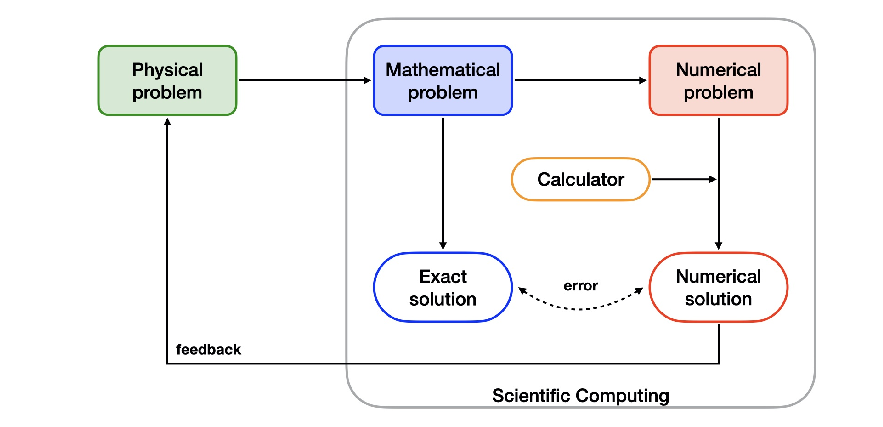
\includegraphics[width=\textwidth]{img/models-1.pdf}
    \caption{Scientific Computing.}
    \label{fig: scientific computing}
\end{figure}
    \subsection{Differential Models and PDEs}

\begin{definitionbox}[: Partial Differential Equation (PDE)]
    A \textbf{differential equation} (model) is an equation that involves \textbf{one or more derivatives of an unknown function}. In an \textbf{Ordinary Differential Equation} (ODE), \textbf{every derivative of the unknown solution is with respect to a single independent variable}. If instead, derivatives are partial, then we have a \definition{Partial Differential Equation (PDE)}.
\end{definitionbox}

\noindent
In other words, it is a differential equation where its derivatives are partial.

\highspace
There are different types of PDEs, and their nature depends on the conditions and their type. Mathematically, we can represent a \textbf{differential model} (equation) as follows:
\begin{equation}
    \mathcal{P}\left(u; g\right) = 0 \hspace{2em} \text{differential equation (mathematical problem)}
\end{equation}
Where:
\begin{itemize}
    \item $\mathcal{P}$ indicates the \emph{\textbf{model}};
    \item $u$ is the \emph{\textbf{exact solution}}, a function of one or more independent variables (space and/or time variables);
    \item $g$ indicates the \emph{\textbf{data}}.
\end{itemize}

\newpage

\subsubsection{ODEs}

\definition{Ordinary Differential Equation (ODE)} is also known as \textbf{initial value problem}.\index{Initial value problem}

\highspace
\begin{flushleft}
    \textcolor{Green3}{\faIcon{book} \textbf{I\textdegree ODE - Cauchy problem}}
\end{flushleft}
A \textbf{first order} ODE, a \textbf{Cauchy problem}, is a differential problem, whose:
\begin{itemize}
    \item \textbf{\emph{Solution}} $u = u\left(t\right)$ is a function of a single independent variable $t$, often interpreted as time.
    \item A \textbf{\emph{single condition}} is assigned on the solution, at a point (usually, the left end of the integration interval).
\end{itemize}
Its form is the following find $u : I \subset \mathbb{R} \rightarrow \mathbb{R}$ such that:
\begin{equation}
    \begin{cases}
        \dfrac{\mathrm{d}u}{\mathrm{d}t}\left(t\right) = f\left(t, u\left(t\right)\right) & t \in I \vspace{1em} \\
        u\left(t_{0}\right) = u_{0}
    \end{cases}
\end{equation}
Where:
\begin{itemize}
    \item $I = \left( t_{0}, t_{f} \right] \subset \mathbb{R}$ is a \emph{\textbf{time interval}};
    \item $u_{0}$ is the \emph{\textbf{initial value}} assigned at $t = t_{0}$;
    \item $f: I \times \mathbb{R} \rightarrow \mathbb{R}$
\end{itemize}
\textcolor{Green3}{\faIcon{question-circle} \textbf{Meaning}}. The equation describes the \textbf{evolution of a scalar quantity $u$ over time $t$}, \textbf{without distribution in space}.

\highspace
\textcolor{Green3}{\faIcon{question-circle} \textbf{Vectorial problems}}. In vectorial problems, the \textbf{unknown is a vector-valued function} $\mathbf{u} = \mathbf{u}\left(t\right)$, where $\mathbf{u} = \left(u_{1}, \dots, u_{m}\right) \in \mathbb{R}^{m}$, with $m \ge 1$. The first order Cauchy problem reads: find $\mathbf{u} : I \subset \mathbb{R} \rightarrow \mathbb{R}^{m}$ such that:
\begin{equation*}
    \begin{cases}
        \dfrac{\mathrm{d}\mathbf{u}}{\mathrm{d}t}\left(t\right) = \mathbf{f}\left(t, \mathbf{u}\left(t\right)\right) & t \in I \vspace{1em} \\
        \mathbf{u}\left(t_{0}\right) = \mathbf{u}_{0}
    \end{cases}
\end{equation*}
Where $\mathbf{u}_{0} \in \mathbb{R}^{m}$ is the initial datum and $\mathbf{f}: I \times \mathbb{R}^{m} \rightarrow \mathbb{R}^{m}$.

\highspace
\begin{flushleft}
    \textcolor{Green3}{\faIcon{book} \textbf{II\textdegree ODE - Cauchy problem}}
\end{flushleft}
A \textbf{second order Cauchy problem} sees second order time derivatives and two initial conditions. It reads as: find $u: I \subset \mathbb{R} \rightarrow \mathbb{R}$ such that:
\begin{equation}
    \begin{cases}
        \dfrac{\mathrm{d}^{2}u}{\mathrm{d}t^{2}}\left(t\right) = f\left(t, u\left(t\right), \dfrac{\mathrm{d}u}{\mathrm{d}t}\left(t\right)\right) & t \in I \vspace{1em} \\
        \dfrac{\mathrm{d}u}{\mathrm{d}t}\left(t_{0}\right) = v_{0} \vspace{1em} \\
        u\left(t_{0}\right) = u_{0}
    \end{cases}
\end{equation}
Where the initial data are $u_{0}$ and $v_{0}$, while $f: I \times \mathbb{R} \times \mathbb{R} \rightarrow \mathbb{R}$.
    \subsubsection{PDE, boundary value problem in 1D}

The \definition{Boundary value problem in 1D} is characterized by a \textbf{single independent variable} $x$, which represents the \textbf{space coordinate in an interval} $\Omega = \left(a,b\right) \in \mathbb{R}$ (1D).

\highspace
The problem involves \textbf{second order derivatives of the unknown solution} $u = u\left(x\right)$ with respect to $x$. The value of $u$, or the \textbf{value of its first derivate}, is a \textbf{set at the two boundaries of the domain} (interval) $\Omega$, that is at $x = a$ and $x = b$ (the domain boundary is $\partial\Omega = \left\{a,b\right\})$.

\highspace
Let us consider the following Poisson problem with (homogeneous) Dirichlet boundary conditions: find $u : \Omega \subset \mathbb{R} \rightarrow \mathbb{R}$ such that:
\begin{equation}
    \begin{cases}
        -\dfrac{\mathrm{d}^{2}u}{\mathrm{d}x^{2}}\left(x\right) = f\left(x\right) & x \in \Omega = \left(a,b\right) \vspace{1em} \\
        %
        u\left(a\right) = u\left(b\right) = 0
    \end{cases}
\end{equation}
This equation models a \textbf{stationary phenomenon} (the time variable doesn't appear in fact) and represent a \textbf{diffusion model}.

\highspace
\begin{examplebox}
    For example, the diffusion model models the diffusion of a pollutant along a 1D channel $\Omega = \left(a,b\right)$ or the vertical displacement of an \emph{elastic thread} fixed at its ends. In the first case, $f = f\left(x\right)$ indicates the source of the pollutant along the flow, while in the second case, $f$ is the traverse force acting on the elastic thread, in the hypothesis of negligible mass and small displacements of the thread.
\end{examplebox}

\noindent
\begin{flushleft}
    \textcolor{Green3}{\faIcon{balance-scale} \textbf{Boundary value problem in 1D vs ODE}}
\end{flushleft}
We remark that the \textbf{boundary value problem in 1D is a particular case of PDEs}, even if it involves only derivatives with respect to a single independent variable $x$. Indeed, even if apparently similar to a second order ODE, the boundary value problem is in reality substantially \textbf{different} from an ODE:
\begin{itemize}
    \item In ODE, two conditions are set at $t = t_{0}$;
    \item In the boundary value problem in 1D, one condition is set at $x = a$ and the other one at $x = b$.
\end{itemize}
The conditions in the boundary value problem determine to the so-called global nature of the model.
    \subsubsection{PDE, initial and boundary value problem in 1D}

\definition{Initial and boundary value problem in 1D} is a type of problems that concern equations that \textbf{depend on space and time}:
\begin{itemize}
    \item The \textbf{unknown solution} $u = u\left(x,t\right)$ both depends on the space coordinate $x \in \Omega \subset \mathbb{R}$ in 1D;
    
    \item The \textbf{time variable} $t \in I \subset I$.
\end{itemize}
In this case, the initial conditions at $t = 0$ must be prescribed, as well as the boundary conditions at the ends of the interval in 1D.

\highspace
The \definition{Heat equation}, also known as \definition{Diffusion equation}, with Dirichlet boundary conditions assumes the following form: find $u: \Omega \times I \rightarrow \mathbb{R}$ such that:
\begin{equation}
    \begin{cases}
        \dfrac{\partial u}{\partial t}\left(x,t\right) - \mu \dfrac{\partial^{2}u}{\partial x^{2}}\left(x,t\right) = f\left(x,t\right) & x \in \Omega = \left(a,b\right), t \in I \vspace{1em} \\
        %
        u\left(a,t\right) = u\left(b,t\right) = 0 & t \in I \\
        %
        u\left(x, t_{0}\right) = u_{0}\left(x\right) & x \in \Omega = \left(a,b\right)
    \end{cases}
\end{equation}

\begin{examplebox}
    For example, the unknown function $u \left(x,t\right)$ describes the temperature in a point $x \in \Omega = \left(a,b\right)$ and time $t \in I$ of a metallic bar covering the space interval $\Omega$. The diffusion coefficient $\mu$ represents the thermal response of the material and it is related to its thermal conductivity. The Dirichlet boundary conditions express the fact that the ends of the bar are kept at a reference temperature (zero degrees in this case), while at time $t = t_{0}$ the temperature is assigned in each point $x \in \Omega$ through the initial function $u_{0}\left(x\right)$. Finally, the bar is subject to a heat source of linear density $f\left(x,t\right)$.
\end{examplebox}

    %%%%%%%%%%%%%%%%%%%%%%%%%%
    % Bibliography and index %
    %%%%%%%%%%%%%%%%%%%%%%%%%%
    \pagestyle{fancy}
\fancyhead{} % clear all header fields
\fancyhead[R]{\nouppercase{\leftmark}}

\bibliography{bibtex}{}
\bibliographystyle{plain}

\newpage

\printindex
\end{document}